\documentclass[aspectratio=169]{beamer}
\usepackage{color,amsmath}
\usepackage{subfigure}
\usepackage{booktabs}
\usepackage{framed}
\usepackage{comment}

\def\vf{\vfill}

%%%%%%%%%%%%%%%%%%%%%%%%%%
\title[]{Approximating experiments (02-06)}
\author[]{Matthew J. Salganik\\Department of Sociology\\Princeton University}
\date[]{Soc 596: Computational Social Science
\vfill
\begin{flushright}
\vspace{0.6in}

\includegraphics[width=0.1\textwidth]{figures/cc.png}
\end{flushright}
}
\begin{document}
%%%%%%%%%%%%%%%%%%%%%%%%%%
\frame{\titlepage}
%%%%%%%%%%%%%%%%%%%%%%%%%%
\begin{frame}

\begin{center}
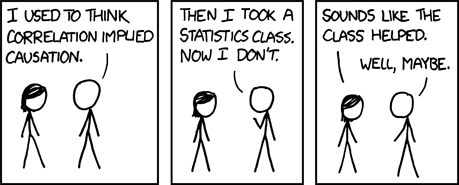
\includegraphics[width=\textwidth]{figures/correlation.png}
\end{center}

\vf
\Tiny{\url{https://xkcd.com/552/}}

\end{frame}
%%%%%%%%%%%%%%%%%%%%%%%%%%
\begin{frame}

\begin{center}
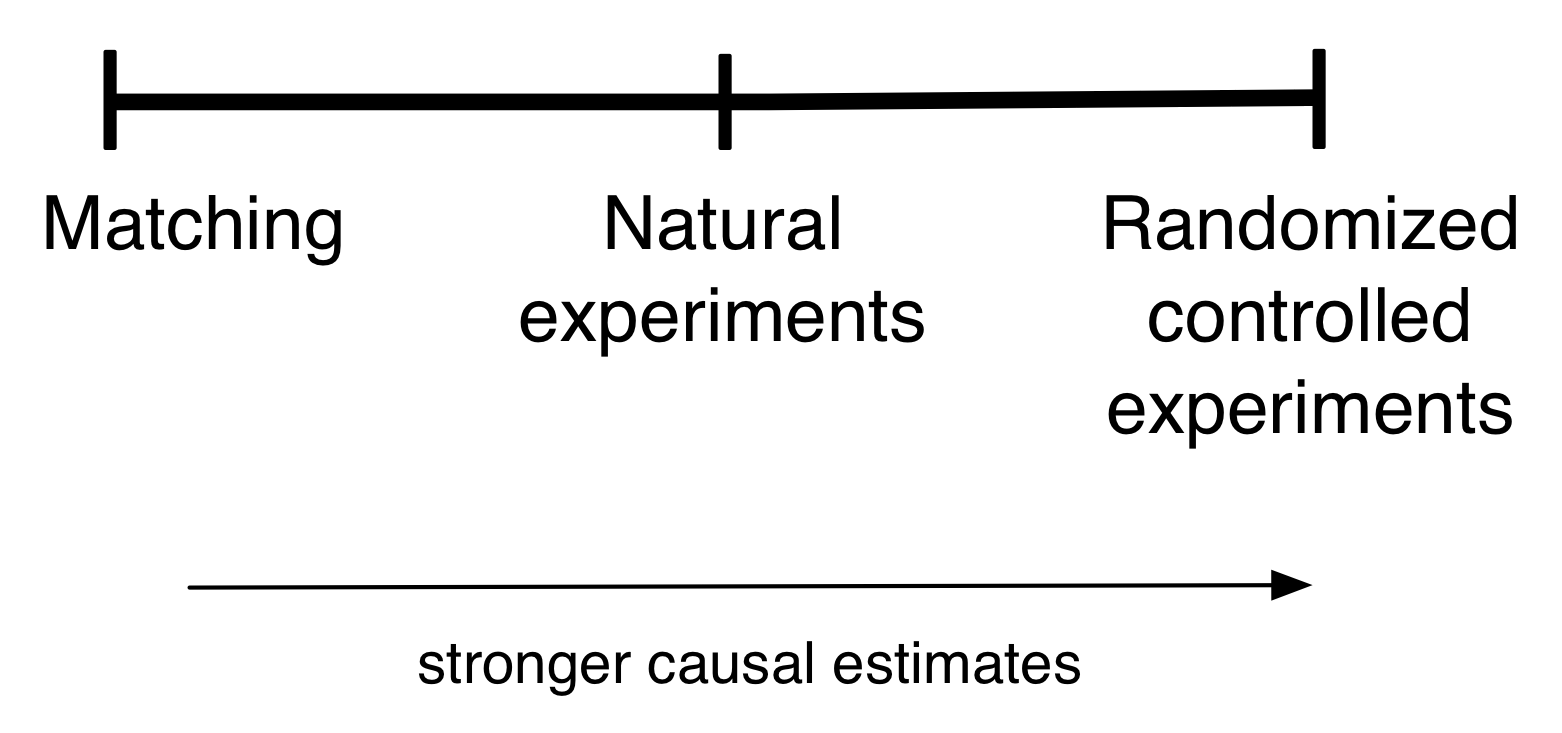
\includegraphics[width=\textwidth]{figures/causal_continuum.png}
\end{center}

\vf
Natural experiments and matching are helped by big data environment

\end{frame}
%%%%%%%%%%%%%%%%%%%%%%%%%%
\begin{frame}

\begin{center}
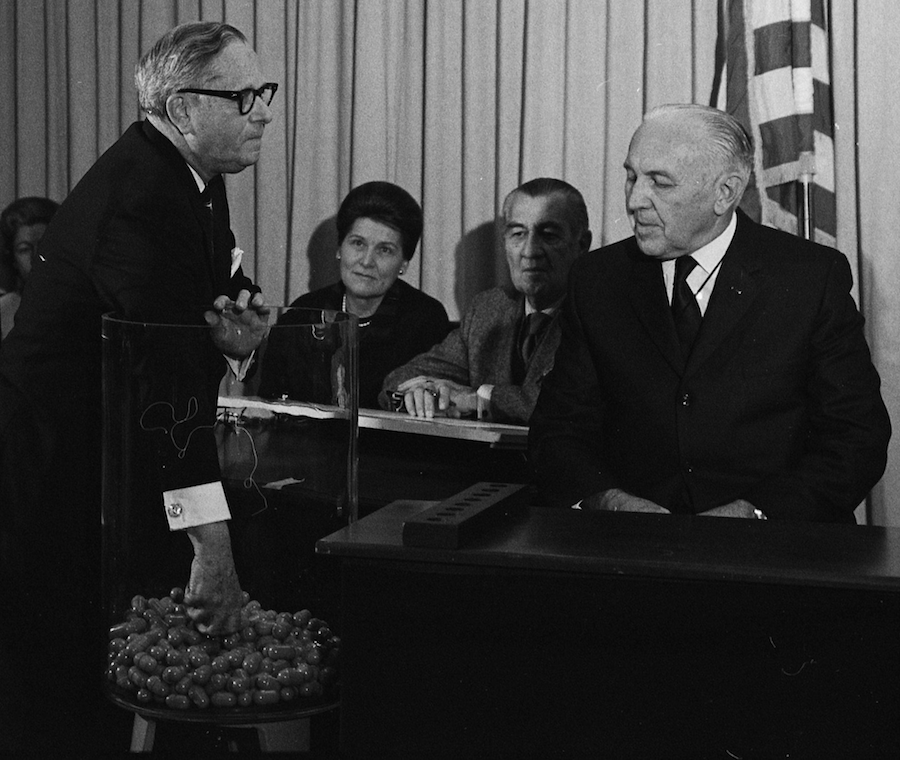
\includegraphics[width=0.6\textwidth]{figures/draft_lottery.png}
\end{center}

\vf
\Tiny{\url{https://commons.wikimedia.org/wiki/File:1969_draft_lottery_photo.jpg}}

\end{frame}
%%%%%%%%%%%%%%%%%%%%%%%%%%
\begin{frame}

Always-on data source + random shock = natural experiment

\end{frame}
%%%%%%%%%%%%%%%%%%%%%%%%%%
\begin{frame}

\begin{center}
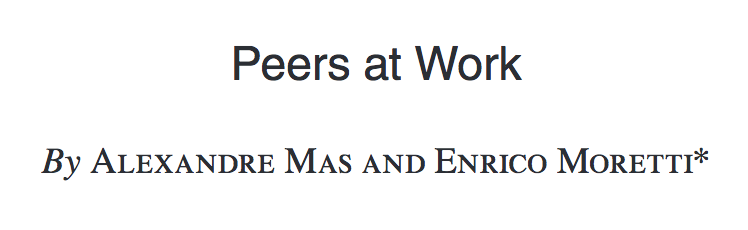
\includegraphics[width=\textwidth]{figures/mas_peers_2009_title}
\end{center}

\vf
Mas and Morietti (2009) ``Peers at works'', \textit{American Economic Review}, \url{http://dx.doi.org/10.1257/aer.99.1.112}

\end{frame}
%%%%%%%%%%%%%%%%%%%%%%%%%%
\begin{frame}

Like Farber (2015)
\begin{itemize}
\item this paper brings a lot of ideas to the data
\item interesting either way (free riding or positive spillovers)
\item both not online (digital devices in the physical world)
\item uses size for heterogeneity and mechanisms
\end{itemize}

\end{frame}
%%%%%%%%%%%%%%%%%%%%%%%%%%
\begin{frame}

\begin{center}
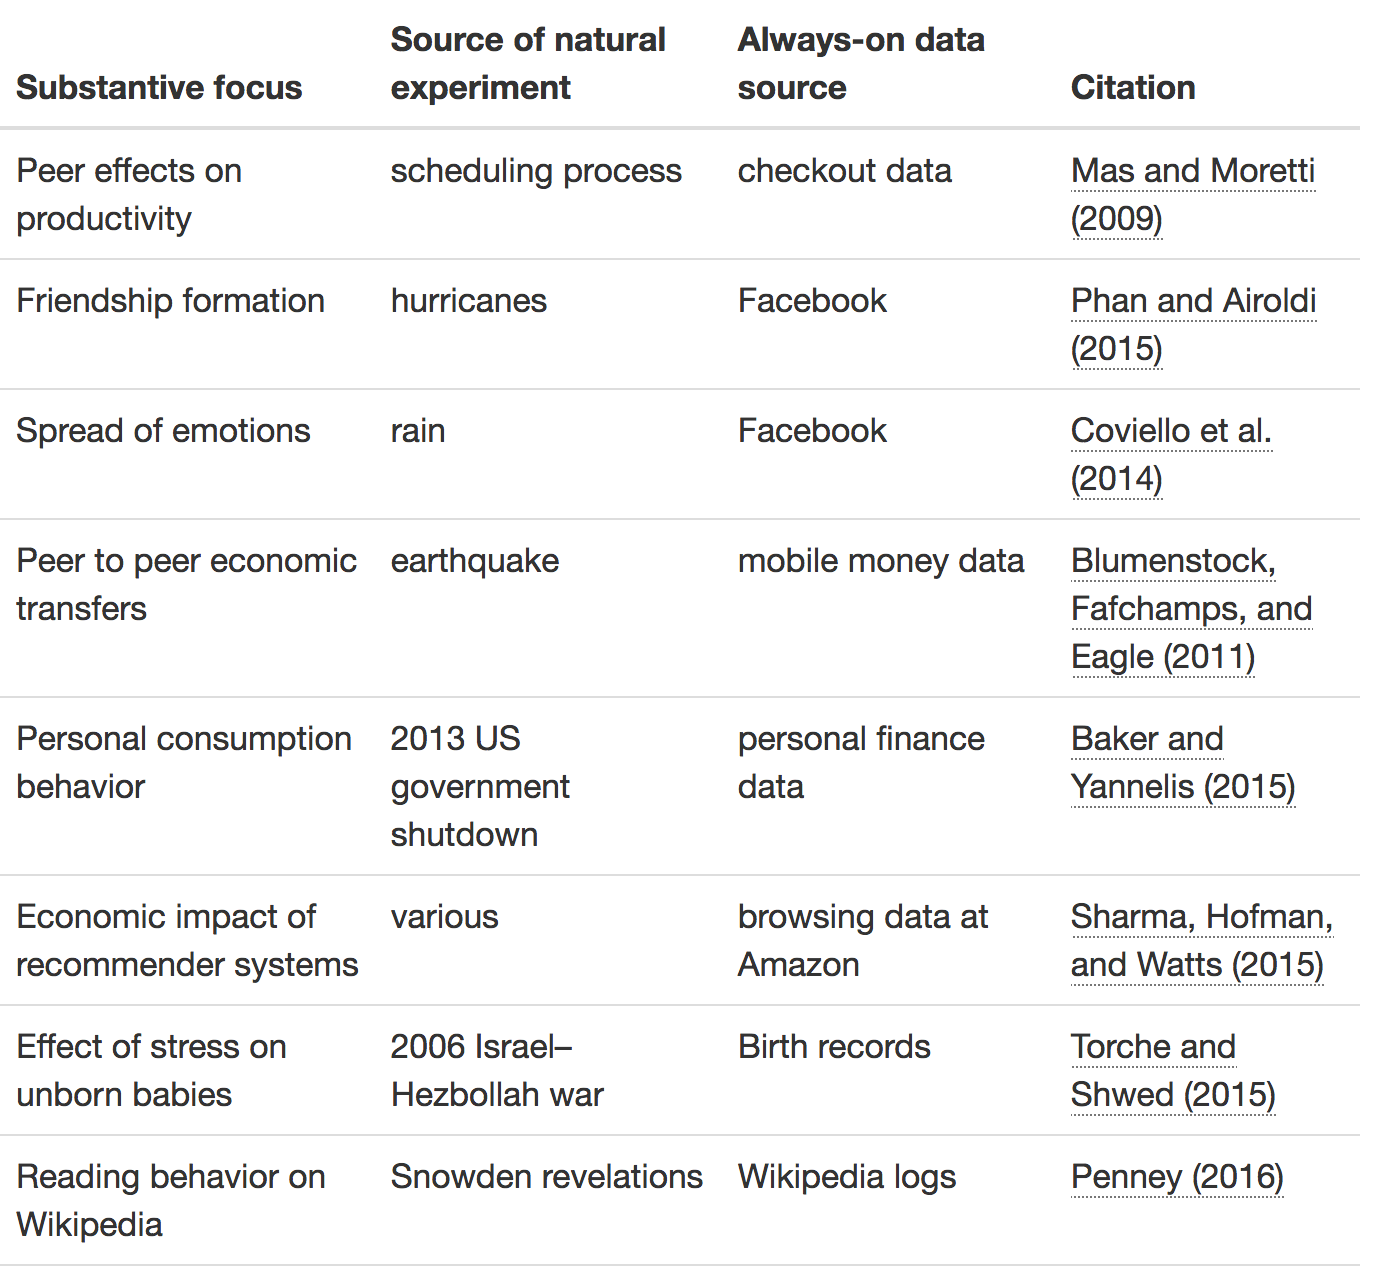
\includegraphics[height=0.8\textheight]{figures/natural_experiments_table.png}
\end{center}

\end{frame}
%%%%%%%%%%%%%%%%%%%%%%%%%%
\begin{frame}

Matching

\end{frame}
%%%%%%%%%%%%%%%%%%%%%%%%%%

\end{document}
